\documentclass[a4paper, onecolumn, 11pt, titlepage]{quantumarticle}
\pdfoutput=1
% \documentclass{article}
\usepackage{graphicx} 
\usepackage{amsmath}
\usepackage{amssymb}
\bibliographystyle{plain} 
\usepackage{hyperref}
\usepackage[toc,page]{appendix}
\usepackage{qcircuit}
\hypersetup{
    colorlinks=true,
    linkcolor=blue,
    filecolor=magenta,      
    urlcolor=cyan,
    pdftitle={Assessing Distant Qubit Entanglement via the CHSH Inequality in Noisy Quantum Environments},
    pdfpagemode=FullScreen,
}

\title{Assessing Distant Qubit Entanglement via the CHSH Inequality in Noisy Quantum Environments}
\author{Adam Jurkowski, Mark Agib, Seaena Kim}
\date{July 2025}

\begin{document}
\maketitle

\begin{abstract}
    Entanglement is the cornerstone of quantum computation and is essential in quantum algorithms. Generating long-range and high-quality entanglement is a necessary milestone for current hardware to reach. We attempt to quantify the quality of entanglement on a quantum computer for distant qubits using Clauser-Horne-Shimony-Holt (CHSH) inequality violations. This is done through simulations on a full circuit noise model using distances ranging from $2$ to $12$.
\end{abstract}



\section{Introduction}
Until the mid-1900s, the principle of locality, stating that objects are solely influenced by their immediate surroundings, remained unquestioned. In 1935, Einstein, Podolsky, and Rosen established the EPR paradox, which exposed quantum mechanics’ violation of the principle of locality, opening up theories of local hidden variables \cite{PhysRev.47.777}. The paradox suggested that current quantum theory implied nonlocal effects, which he famously called "spooky action at a distance." In order to resolve this problem, EPR proposed the idea of local hidden variables that would preserve locality and determinism. However, EPR was challenged by John Stweart, who introduced mathematical inequalities, and it offered an experimental violation that would rule out EPR's theory of hidden variables and confirm the presence of non-local quantum correlations \cite{PhysicsPhysiqueFizika.1.195}. Subsequent experiments, like that of Clauser-Horne-Shimony-Holt (CHSH) formulation of Bell's theorem, provided increasing support of quantum mechanics and laid the foundation for understanding quantum entanglement. 

This paper aims to investigate the CHSH version of Bell's inequalities to quantify the quality of entanglement between distant qubits on quantum processors. Entanglement is essential for any application of quantum computing, such as quantum teleportation, quantum key distribution, quantum algorithms, and more. As such, ensuring that Noisy Intermediate Scale Quantum (NISQ) devices can successfully create high-quality entanglement is necessary for the success of the field. 

\section{Literature Review}

John Clauser and Stuart Freedman were the first to test Bell’s inequalities in 1972. A researcher at UC Berkeley, Clauser, explored entangled photons with graduate student Freedman \cite{PhysRevLett.28.938}. Before the experiment, Clauser and his colleagues, Michael Horne, Abner Shimony, and Richard Holt, created the CHSH inequality, a variant of Bell’s theorem, as a way to experimentally test Bell’s original inequality \cite{PhysRevLett.23.880}. The CHSH inequality is as follows:

\begin{equation} \label{eq1}
\begin{split}
    S & \leq 2
\end{split}
\end{equation}
such that 
\begin{equation} \label{eq2}
\begin{split}
    S & = E(A,B) - E(A, B') +E(A', B) + E(A', B')
\end{split}
\end{equation}

Suppose $A$ and $B$ are Alice and Bob at opposite ends of a certain distance. Alice and Bob each have their two observables $(a, a’)$ and $(b, b’)$ that measure qubits. 4 distinct combinations are possible from the 4 measurements. Each term, such as $E(a,b)$, represents the quantum correlations of the four pairs, where $E()$ calculates the average of the products of the pairs over multiple runs. If the value $S$ is either less than $-2$ or greater than $2$, the particles are in entangled states and do not behave under theories of locality or hidden variables. 

There are four crucial elements of understanding quantum circuits and mechanics: Entanglement, Superposition, Interference, and Measurement. Entanglement is what Bell's equation and CHSH focus on the most, where two or more qubits become intertwined with each other and are able to exchange information instantaneously. Superposition is when a qubit is in two or more states, positions, or phases at once. For instance, a coin can be both heads and tails until physically measured. Interference occurs when qubits add or subtract, meaning their wave-like behavior causes qubits to augment or cancel each other out. Measurement takes away the quantum behavior of a qubit to cater to how people can see them. Therefore, measuring causes qubits in superposition, like the plus state, to collapse into one state, either 1 or 0. These quantum fields are hard to explore even today due to environmental noise and the delicacy of quantum entanglement and superposition circuits. 

In Clauser and Freedman’s experiment, they utilized polarized photons from calcium atoms instead of Bell’s original intended electrons. These particles, called $\gamma_1$and $\gamma_2$, were measured $10$ feet apart and viewed by optical systems made up of two lenses, a wavelength filter, a removable and rotatable polarizer, and a single-photon detector. The following diagram (\hyperref[fig:system-diagram]{Figure 1}) depicts the system that Clauser and Freedman used: 

\begin{figure}
    \centering
    \includegraphics[width=1.0\textwidth]{figs/pic1.png}
    \caption{Experimental apparatus for the 1972 test of Bell’s theorem using polarization-entangled photon pairs ($\gamma_1$, $\gamma_2$) from a calcium atomic cascade. Photons travel 10 feet through independent optical systems, each consisting of a lens, polarization filter (rotatable), wavelength filter, and single-photon detector. Coincidence rates $R(\varphi)$ and relative polarization angle $\varphi$ are recorded, testing the predictions of quantum mechanics against local hidden-variable theories.}
    \label{fig:system-diagram}
\end{figure}

The two detectors recorded two variables: coincidence rate of two-photon detection $[R(\varphi)]$ and the angle of the planes of linear polarization $[\varphi]$. If these particles behaved according to quantum mechanics, its behavior would invalidate local hidden-variable theory and reject Bell’s inequality which assumes the following: The two photons propagate as separate localized particles; A binary selection process occurs for each photon at each polarizer; All photons incident on a detector have a probability of detection that is independent of whether or not the photon has passed through a polarizer. Mathematically, these assumptions create the following inequalities:

$$-1 \leq \Delta(\varphi) \leq 0$$
where
$$\Delta(\varphi) = \frac{3R(\varphi)}{R_0} - \frac{R(3\varphi)}{R_0} - \frac{R_1+R_2}{R_0}$$

The following graph (\hyperref[fig:angles-graph]{Figure 2}) shows the quantum correlation between the coincidence rate defined by the angle of the polarizers, divided by the rate with both polarizers removed, and the angle. 

\begin{figure}
    \centering
    \includegraphics[width=1.0\textwidth]{figs/pic2.png}
    \caption{Quantum correlation $\Delta(\varphi)$ vs. polarizer angle $\varphi$, showing violation of Bell’s inequality and agreement with quantum mechanics.}
    \label{fig:angles-graph}
\end{figure}

Using the CHSH Bell inequality and quantum mechanics, Clauser and Freedman were able to conclude that the behavior of these particles, measured by polarizer efficiencies and angles, rejected local hidden variable theories and upheld principles of entanglement. 
Since Clauser and Freedman’s experiment, scientists have used Bell’s inequalities to further back up quantum physics and theories. These experiments are performed to explore the utility of quantum-behaved particles and potentially find a way to send information over these qubits. In our experiment, we will utilize a quantum circuit and Bell’s inequality to find a way to efficiently send information over a certain distance without being intercepted by noise or other environmental factors. 


% lit rev2 
\subsection{CHSH for Quantum Computation}

% In Bartkiewicz, Horst, Lemr, and Miranowicz’s experiment, they explored extremal states of quantum mechanics. While the CHSH inequality is useful for testing the quantum behavior of some particles, there are extremes where particles can be entangled, but still abide by the CHSH inequality. Similar to the EPR paradox, particles can follow classical-leaning theorems, while having quantum characteristics such as entanglement. 
% In the research paper Entanglement estimation from Bell inequality violation, scientists Bartkiewicz, Horst, Lemr, and Miranowicz used the CHSH inequality to explore states of 
% particles that have quantum characteristics but do not violate the inequality. These states are known as Werner states and are applied to the following equation: 

% $$\rho_W = p|\Psi^-\rangle \langle\Psi^-| + \frac{1 - p}{4}I \otimes I$$

% where $|\Psi^-\rangle$ is the bell state $|\Psi^-\rangle = \frac{1}{\sqrt{2}} (|01\rangle - |10\rangle)$ and $p \in [0,1]$. 
%  The CHSH inequality is violated when 
% $\frac{1}{\sqrt{2}} < p \leq 1$
% The particles are entangled when 
% $\frac{1}{3} < p \leq 1$.
% Therefore, while $\frac{1}{3} < p \leq \frac{1}{\sqrt{2}}$, the states are entangled and satisfy the CHSH inequality. 
% The Karush-Kuhn-Tucker conditions, otherwise known as the saddle-point theorem, are applied to nonlinear programming in order to utilize the constrained optimization problem with inequalities. The four scientists used the KKT conditions as well as Lagrange multipliers which find the maximum and minimum values of a function (extremal states). From here, they explored the different concurrences of specific classes of qubits of two-qubit states. Using Monte Carlo simulations and the Horodecki measure, Bartkiewicz, Horst, Lemr, and Miranowicz were able to experiment with the boundaries of Bell’s inequality and entanglement. 
% From this paper, we learned to acknowledge the limitations of the CHSH inequality while collecting our qubit circuit data. 


Violation of the CHSH inequality has become a popular approach to measure entanglement on various types of quantum computers (quantum dot \cite{steinacker2025bell}, superconducting \cite{storz2023loophole}) and different types of matter. The first experimental validation of the Bell-CHSH inequality on a major quantum computer was done on IBM’s $5$ qubit computer in 2016. Many years later, the inequality still serves as one of the first measures of entanglement for any new quantum computer as proof of quantum mechanical properties. Besides the CHSH inequality, the three most common entanglement measures are negativity \cite{PhysRevA.65.032314}, concurrence \cite{PhysRevLett.80.2245}, and Relative Entropy of Entanglement (REE) \cite{PhysRevLett.78.2275}. While CHSH inequality violation is a great way to quantify the quality of entanglement, there remain states like the Werner states that show entanglement yet do not always violate the CHSH inequality. They are written as:
$$\rho_W = p|\Psi^-\rangle \langle\Psi^-| + \frac{1 - p}{4}I \otimes I$$

where $|\Psi^-\rangle$ is the bell state $|\Psi^-\rangle = \frac{1}{\sqrt{2}} (|01\rangle - |10\rangle)$ and $p \in [0,1]$. 
 The CHSH inequality is violated when 
$\frac{1}{\sqrt{2}} < p \leq 1$
The particles are entangled when 
$\frac{1}{3} < p \leq 1$.
Therefore, while $\frac{1}{3} < p \leq \frac{1}{\sqrt{2}}$, the states are entangled, but do not violate the inequality. 


% Incomplete
Most recently, a short study conducted in 2025 used CHSH violations to explore the success of different CNOT implementations across distant qubits on \verb|ibm_qubec| \cite{waring2025chshviolationsusingdynamic}. As the distance between the entangled qubits rose, the CHSH Parameter (S) fell as expected. They found that the "post-processing" method of generating a CNOT was the most successful, and higher fidelity readout measurements would be necessary to achieve better results.

Our work aims to answer the question: \textit{How can the CHSH parameter be used to measure the quality of entanglement on distant qubits based on noisy simulations of quantum computers?} We answer this question with a method similar to \cite{waring2025chshviolationsusingdynamic} using noisy simulations based on real IBM Quantum backends.

\section{Method}

We used the library \verb|Qiskit|’s AerSimulator \cite{qiskit2024} to simulate the created circuits using noise models from real IBM Quantum backends (see code in \hyperref[secondappendix]{Appendix B}. Before the circuits are simulated, they need to be “transpiled”, which means translated to fit the topology of the specific device and for optimization on the specific hardware. For our case, when \verb|optimization_level=3|, which is the highest level of optimization, and we finally mapped the qubits to be neighboring each other using a coupling map, which maps connections of qubits (ex: \hyperref[fig:coupling-map]{Figure 3}). 

\begin{figure}
    \centering
    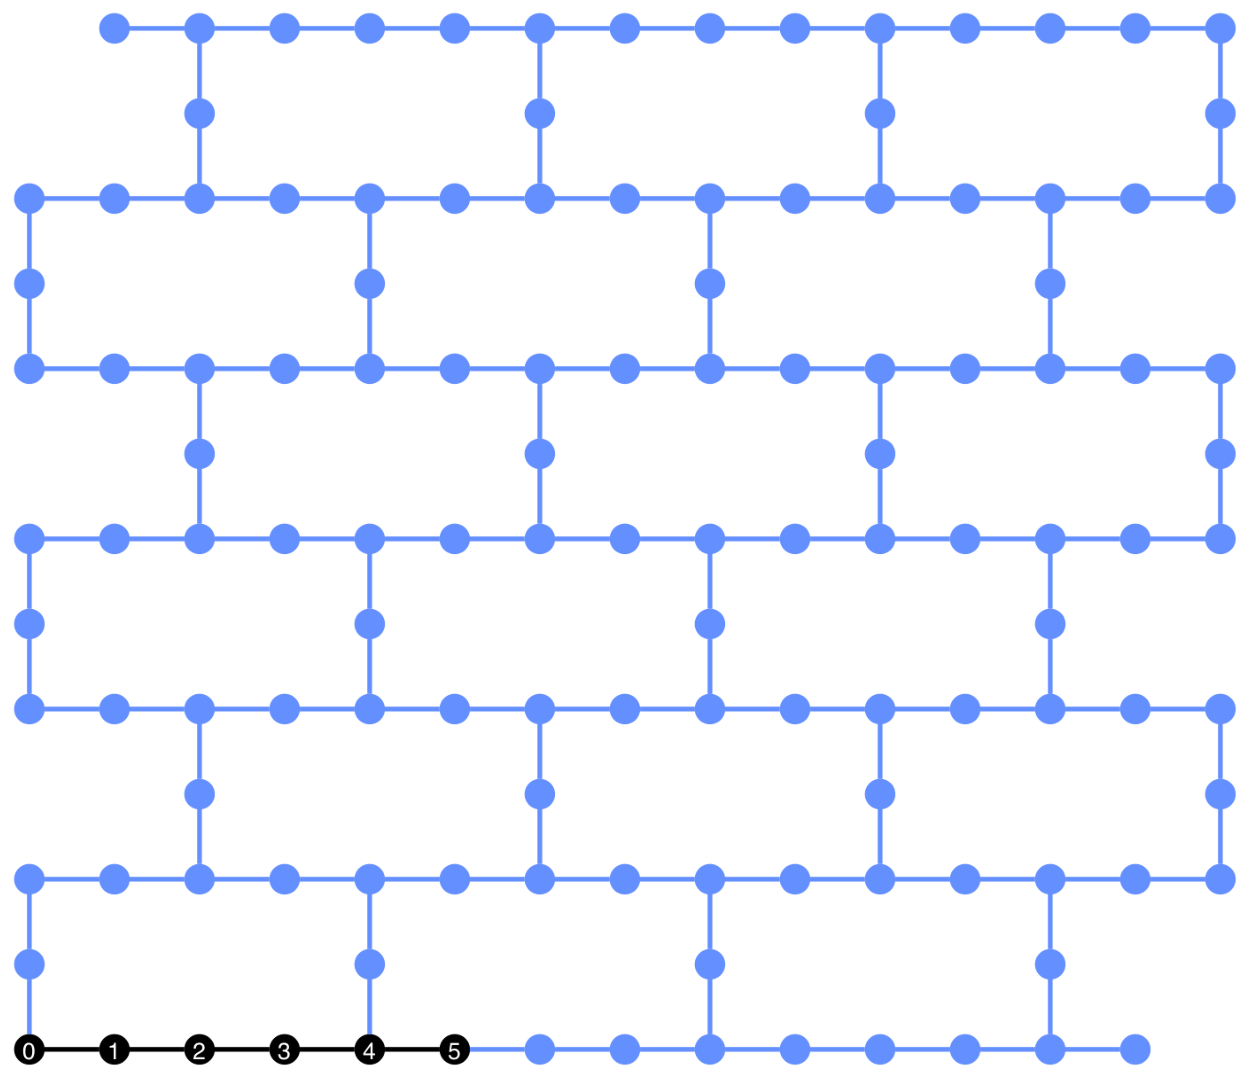
\includegraphics[width=1.0\textwidth]{figs/coupling_map.png}
    \caption{The coupling map of \texttt{ibm\_brisbane}'s  $127$ qubits on the Eagle r3 processor is shown above. In the bottom left are the $6$ qubits used in a sample CHSH circuit.}
    \label{fig:coupling-map}
\end{figure}


\begin{figure}
    \centering
    \scalebox{1.25}{
        \[
            \Qcircuit @C=1em @R=1em {
            \lstick{\left| 0 \right\rangle} & \gate{H}  & \ctrl{1} \barrier[0em]{1} & \qw & \gate{H}  \barrier[0em]{1} & \qw & \meter  \\
            \lstick{\left| 0 \right\rangle} & \qw & \targ & \qw & \gate{R_y(\phi)} & \qw  &  \qw & \meter \\
            & \cw & \cw & \cw & \cw & \cw & \cw \cwx[-2] & \cw \cwx[-1] & \cw \\
            }
        \] 
    }
    \caption{An example circuit that would violate the CHSH inequality, where the top qubit is "Alice's" and the lower is "Bob's" qubit. We always begin with initializing the bell state (shown in the first section) and follow with a change of measurement basis based on the inputs. In the circuit shown above, Alice and Bob have received $x = 1$ and $y = 1$, respectively, creating their appropriate measurement bases. }
    \label{fig:circuit-basic}
\end{figure}

For the construction of our circuits, we began by creating a Bell state between the two qubits that would be Alice's and Bob’s, and then we applied different gates (based on the inputs) to change the measurement basis. When Alice was given a $0$, she would measure on a regular $Z$ basis, and given a $1$, she would measure on an $X$ basis (hence we apply a Hadamard). Traditionally the CHSH parameter’s value is maximized when Bob’ measures in the $\frac{Z+X}{\sqrt2}$ basis when given $0$ and $\frac{Z-X}{\sqrt2}$ basis when given $1$, which translates to $\frac{\pi}{4}$ rotations in the y-axis (see the example circuit in \hyperref[fig:circuit-basic]{Figure 4}). 

In our case we tested 43 different phases between $\frac{\pi}{2}$ to $3\pi$. We chose 43 phases because it was the only number of phases between 31 and 100 that equally spaced intervals would include the optimal phase $\frac{\pi}{4}$. We also test on three different noise models (using \verb|NoiseModel.from_backend(backend)|) for the three backends: \verb|ibm_brisbane|, \verb|ibm_torino|, and \verb|ibm_sherbrooke|, which all have a heavy hex topology. The only difference is the processor, \verb|ibm_torino| has the Heron R1, and the rest have the Eagle R3. For each noise model, we try distances from $2$ qubits (standard circuit) to $12$ qubits.



\begin{figure}
    \centering
    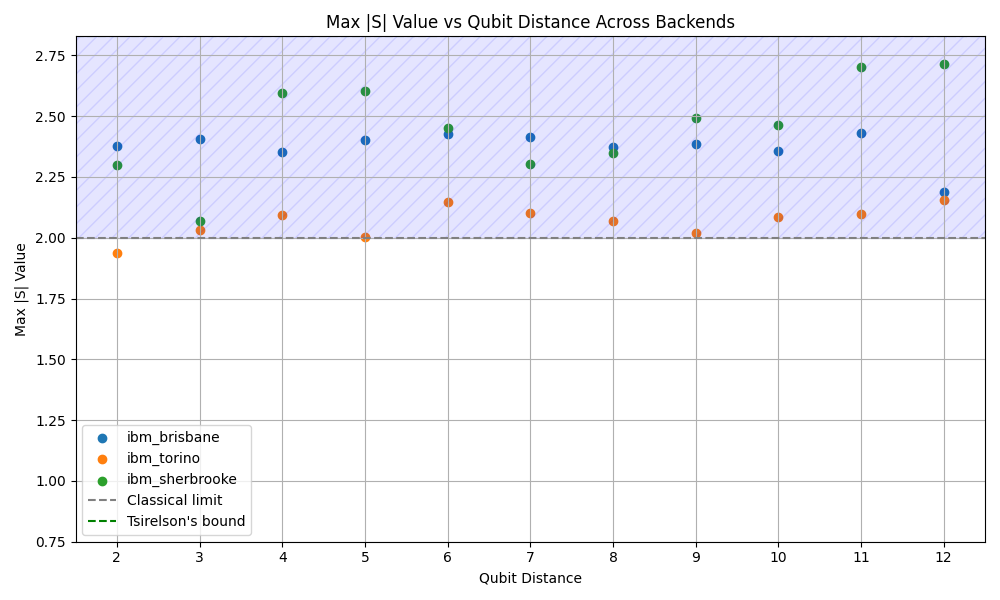
\includegraphics[width=1.0\textwidth]{figs/max vs qubit distance.png}
    \caption{Entangling qubits from $2$ (neighboring qubits) up to $12$ (10 qubits in between) for the backends: \texttt{ibm\_brisbane} (blue dots), \texttt{ibm\_torino} (orange dots), and \texttt{ibm\_sherbrooke} (green dots). On the y-axis is the $\max|S|$ value found after running the corresponding circuit. The blue shaded region from $2$ to $2\sqrt{2}$ is where the CHSH inequality is violated; the closer the value to $2\sqrt{2}$, the better quality the entanglement.}
    \label{fig:all}
\end{figure}

\begin{figure}
    \centering
    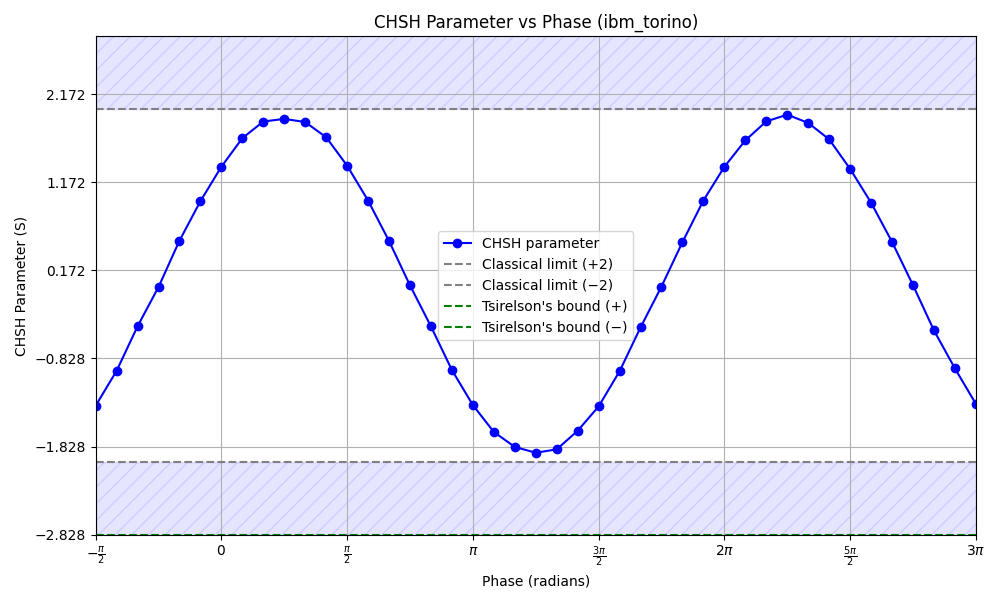
\includegraphics[width=1.0\textwidth]{figs/torino_anamoly.png}
    \caption{A graph of phase values vs the CHSH Parameter $S$. The areas where the CHSH inequality is violated are shaded in blue ($2$ to $2\sqrt{2}$). This graph was created as a result of running a CHSH violating circuit between neighboring qubits using the \texttt{ibm\_torino} noise model. Even at the optimal rotation ($\frac{\pi}{4}$), the circuit does not produce an $S$ value greater than 2.}
    \label{fig:torino}
\end{figure}

\section{Discussion}
After running the noisy simulations on three different backends for $11$ distances each, we stored our results in a \verb|.json| file. While we got $43$ different $S$ values, most did not violate the inequality. This was expected because even in noiseless simulations, only certain changes of Bob’s measurement basis can line up with Alice’s measurement basis. The optimal rotation in the y-axis is actually multiples of $\frac{\pi}{4}$ (see \hyperref[firstappendix]{Appendix A}), which is where the circuit usually violates the inequality. 

The results (see in \hyperref[fig:all]{Figure 5}) were slightly unexpected because usually, if the qubit distance is getting larger, it means a deeper circuit is required to entangle the two qubits. This means that, in theory, more errors can occur. This implies that the $\max(|S|)$ should be lower. Interestingly, although \verb|ibm_torino| uses a newer processor, it has more two-qubit errors than the other two smaller backends. Overall, \verb|ibm_sherbrooke| performed the best. We assume that this is not because of the number of repetitions or \verb|SHOTS|, because we used 10000, which means that these results must have been very consistent for them to change the maximum value unexpectedly. The biggest outlier is the `\verb|ibm_torino| maximum $S$ value at $2$ qubits, since this is the base circuit, and yet it performs the worst on it as seen in \hyperref[fig:torino]{Figure 6}. We theorize that these deviations were the cause of heavy amounts of noise, reversing what the actual result should have been, causing the parameter values to appear larger. 

It is also worth noting that, unlike other cases \cite{storz2023loophole}, \cite{steinacker2025bell}, \cite{Zhong_2019}, we did not have to worry about the effects of "loopholes" as we ran a simulation. One must also consider that our method of measuring the violation of the inequality was based on the CHSH game, experimentally realized in \cite{PhysRevLett.49.91} and a first description of non-local games in \cite{cleve2010consequenceslimitsnonlocalstrategies}. Another such way to measure violation in an analytical way using the CHSH inequality is based on Horodecki et al. \cite{HORODECKI1995340, HORODECKI1996223} using Pauli observables \cite{PhysRevA.88.052105}, \cite{Kalaga_2024}. Future researchers are recommended to try using Horodecki measurements, as we theorize they may result in better results under strenuous noise than the CHSH game method.

\section{Conclusions}

The popularization of the CHSH inequality in the late 1900s and early 21st century gave way to many novel experiments, which further enhanced human understanding of quantum physics. Using coding to model the behavior of particles in a quantum space allowed us to make conclusions on how and when particles are in an entangled state. Two variables, Alice and Bob, measure qubits simultaneously and apply gates that effectively increase the value of the CHSH parameter. We measured the qubits in 43 different phases between $[-\frac\pi2, 3\pi]$. After plotting the results on an x-y coordinate graph, there is an evident sinusoidal pattern that tells us at which intervals the CHSH inequality is being invalidated. When the phase was between 0 and 2, the plot points crossed the dotted line at y=2. This means that the S parameter of the CHSH inequality invalidates the rule that S must be less than or equal to 2. Additionally, this pattern occurs in periods of , which helps us understand at which sequences the two particles are entangled. 

Furthermore, we used the Qiskit library to create noise models, \verb|ibm_brisbane|, \verb|ibm_torino|, and \verb|ibm_sherbrooke|, to test the strength of entanglement of particles. We tested the particles at various distances. However, our data suggested that as the distance between the particles increased, the CHSH parameter also increased. This does not make logical sense because the strength of entanglement should theoretically decrease over increasing distance intervals, since the CNOT creating entanglement across qubits would be susceptible to more noise. In our case, the adverse effects of noise seemed to create high-quality entanglement, perhaps coincidentally. 



\newpage
\bibliography{refs}

\newpage{}

\begin{appendices}
\section{Supplementary Information}\label{firstappendix}

\subsection{Why $\frac{\pi}{4}?$}

The reason why $\frac{\pi}{4}$ is the optimal rotation in the y-axis is because of what basis Bob is measuring in. To achieve Tsirelson's bound ($S = 2\sqrt2$), you start in the entangled Bell state and then change the measurement basis based on values of $x$ and $y$. 

The following is based on a \href{ttps://math.ucsd.edu/sites/math.ucsd.edu/files/XiaoFeng.pdf}{proof} by Xiao Feng.

Let Alice have the angles to measure in be $\alpha, \alpha'$, and Bob have $\beta, \beta'$, and they share the Bell state. Then their correlation is
$$E(\alpha, \beta) = cos[2(\alpha -\beta)]$$
and the CHSH parameter becomes:
$$S = cos[2(\alpha -\beta)] - cos[2(\alpha' -\beta)] + cos[2(\alpha -\beta')] - cos[2(\alpha' -\beta')]$$

If we let $\alpha = 0, \alpha = \pi/2$ and $\beta = \theta, \beta' = \theta$ and we subsistue into the CHSH paramter we have:
$$S(\theta) = 4cos(2\theta)$$ 
amd to maximize $S(\theta)$ we need to find where the max of $cos(2\theta)$ occurs. We find that $\theta = \pi$ and $S$ can equal $4$, but this isn't physically realizable, and the max of $S$ is further below that, which is why $\theta$ can only go up to $\frac{\pi}{4}$.

\subsection{Other CHSH Inequality Formalisms}
Some papers denote the CHSH inequality a little differently. It is denoted as 

$$\left|\text{Tr}\left(\rho \mathcal{B}_{CHSH}\right) \right| \leq 2$$

(\textit{Note}: This stems from the fact that the expectation value of an observable is the trace of the density matrix and the observable.)They describe the CHSH parameter or operator as 

$$\mathcal{B}_{CHSH} = \vec{a} \cdot \vec{\sigma} \otimes \left(\vec{b} +\vec{b}' \right) \cdot \vec{\sigma} + \vec{a}' \cdot \vec{\sigma} \otimes \left(\vec{b} - \vec{b}'\right) \cdot \vec{\sigma}$$

where $\vec{a}$, $\vec{a}'$ and $\vec{b}$, $\vec{b}'$ are unit vectors in $\mathfrak{R}^3$ and describe the measurements on Alice and Bob's sides, respectively, and $\sigma$ are vectors of the Pauli matrices. (*Note*: Taking the dot product of Alice's unit vector and the Pauli matrix is an observable, and it corresponds to measuring on the Pauli matrix's axis.) On a further side note (skip ahead if you understand), the correlation functions described in the classic CHSH expression $E(a, b)$ can be written mathematically as 

$E(\vec{a},\vec{b}) = \text{Tr} \left[\rho \left(\vec{a} \cdot \vec{\sigma} \otimes \vec{b} \cdot \vec{\sigma} \right) \right]$

And so when we substitute in for those terms, we get

$$ \text{Tr} \left[ \rho \left(\vec{a} \cdot \vec{\sigma} \otimes \vec{b}\cdot \vec{\sigma} + \vec{a} \cdot \vec{\sigma} \otimes \vec{b}' \cdot\vec{\sigma} + \vec{a}' \cdot \vec{\sigma} \otimes \vec{b} \cdot \vec{\sigma} - \vec{a}' \cdot \vec{\sigma} \otimes \vec{b}' \cdot \vec{\sigma} \right) \right] $$

(pretty long lol). But once we group (try this yourself), we get

$$\vec{a} \cdot \vec{\sigma} \otimes \left(\vec{b} +\vec{b}' \right) \cdot \vec{\sigma} + \vec{a}' \cdot \vec{\sigma} \otimes \left(\vec{b} - \vec{b}'\right) \cdot \vec{\sigma}$$

which happens to be exactly what the CHSH operator was (check for yourself). That's because these are equivalent ways to write the same thing.


And the density matrix $\rho$ can be expressed as 

$$\rho = \frac{1}{4}\left(I\otimes I + \vec{r} \cdot \vec{\sigma} \otimes I + I \otimes \vec{s} \cdot \vec{\sigma} + \sum_{n, m = 1}^{3}{T_{n,m}\sigma_n \otimes \sigma_m}\right) $$

where $T_{n,m} = \text{Tr} \left[\rho \left(\sigma_i \otimes \sigma_j \right)\right]$ is the corrleation matrix and $\vec{r}$ and $\vec{s}$ are unit vectors in $\mathfrak{R}^3$. Now you might be wondering what all that means. Well, it's based on a representation of the Bloch sphere for two qubits. The $I \otimes I$ is the identity operator applied on the first and second qubits. It's then added to the dot product of the Pauli matrices on the unit vector tensored with the identity operator like $(r_1 \sigma_1 +r_2 \sigma_2 + r_3 \sigma_3) \otimes I$ that. You then do the same for the second qubit (on $\vec{s}$).

Finally, in the summation  $\sigma_n \otimes \sigma_m$ is all the possible combinations of Pauli operators on $1$ and $2$ (hence the sum to $3$), and the correlation matrix describes how strongly the qubits are correlated along the axes. Since $ \text{Tr}(\rho) = 1$ the factor $\frac{1}{4}$ keeps the trace $1$.

For the Horodecki measure, we take the method of the CHSH operator $\mathcal{B}_{CHSH}$. Again we define the corelation matrix as $T_{i,j} = \text{Tr} \left[\rho \left(\sigma_i \otimes \sigma_j \right)\right]$. 

And the maximum possible value for the CHSH operator given the density matrix $\rho$ is

$$\max_{\mathcal{B}_{CHSH}}{|\text{Tr}(\rho \mathcal{B}_{CHSH})|} = 2 \sqrt{\mathcal{M}(\rho)}$$

where $\mathcal{M}(\rho) = \max_{i > j}{(u_i +u_j)}$ where $u_i$ are eigenvalues of $T^\dagger T$. And in this representation, the CHSH inequality is only violated iff $\mathcal{M}(\rho) > 1$. We can then define

$$B(\rho) \equiv \sqrt{\mathcal{M}(\rho) - 1}$$ 

Some may also say:

$$B(\rho) \equiv \sqrt{\max[0, \mathcal{M}(\rho) - 1]}$$ 

just so that the $B$ remains a real value function, and we call it the Horodecki measure of the CHSH inequality. Its values range from $0$ to $1$, with larger values meaning more entangled.

Sources: \cite{PhysRevA.88.052105} and \cite{Kalaga_2024}.


\section{Code}\label{secondappendix}
Find the code at: \href{https://github.com/MarkAppprogrammer/CHSH-Ineq/tree/main}{https://github.com/MarkAppprogrammer/CHSH-Ineq/}.
\end{appendices}

\end{document}
